%# -*- coding: utf-8-unix -*-
%%==================================================
\tikzset{every picture/.style={line width=0.75pt}} %set default line width to 0.75pt    

\chapter{波动与光学}

\section{参考圆}

\subsection{定义}

简谐振动中,物体的位移$x$满足正弦规律变化\footnote{这里我们不区分所谓的“正弦式变化”、“余弦式变化”,本质上只是后文提及的初相不同而已},即$x = A \sin (\omega t + \varphi)$,其中,$A$被称之为\textbf{振幅},$\omega = \frac{2 \pi}{T}$被称之为\textbf{频率},$(\omega t + \varphi)$称之为\textbf{相位}(其随时间而变化),而$t=0$时 的相位我们称其为$初相$。

对于一个简谐振动,我们总可以认为其为\textbf{半径为$A$、角速度为$\omega$的匀速圆周运动在$x$轴或者$y$轴上的投影},我们将这个投影后为所需的简谐振动的圆称为\textbf{参考圆}。

\begin{center}


\tikzset{every picture/.style={line width=0.75pt}} %set default line width to 0.75pt        

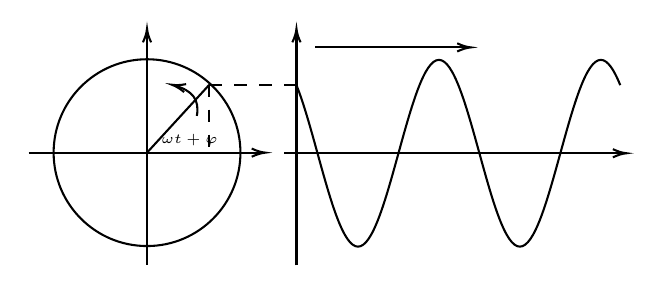
\begin{tikzpicture}[x=0.75pt,y=0.75pt,yscale=-0.6,xscale=0.6]
%uncomment if require: \path (0,300); %set diagram left start at 0, and has height of 300

%Straight Lines [id:da6372713083546984] 
\draw    (65,169.52) -- (253,169.52) ;
\draw [shift={(255,169.52)}, rotate = 180] [color={rgb, 255:red, 0; green, 0; blue, 0 }  ][line width=0.75]    (10.93,-3.29) .. controls (6.95,-1.4) and (3.31,-0.3) .. (0,0) .. controls (3.31,0.3) and (6.95,1.4) .. (10.93,3.29)   ;
%Straight Lines [id:da44936558403337346] 
\draw    (160,72) -- (160,260) ;
\draw [shift={(160,70)}, rotate = 90] [color={rgb, 255:red, 0; green, 0; blue, 0 }  ][line width=0.75]    (10.93,-3.29) .. controls (6.95,-1.4) and (3.31,-0.3) .. (0,0) .. controls (3.31,0.3) and (6.95,1.4) .. (10.93,3.29)   ;
%Shape: Circle [id:dp23986433167584287] 
\draw   (85,169.52) .. controls (85,128.1) and (118.58,94.52) .. (160,94.52) .. controls (201.42,94.52) and (235,128.1) .. (235,169.52) .. controls (235,210.95) and (201.42,244.52) .. (160,244.52) .. controls (118.58,244.52) and (85,210.95) .. (85,169.52) -- cycle ;
%Straight Lines [id:da671297841722321] 
\draw    (210,115) -- (160,169.52) ;
%Straight Lines [id:da5109888412647536] 
\draw  [dash pattern={on 4.5pt off 4.5pt}]  (210,115) -- (210,170) ;
%Straight Lines [id:da0436893772008915] 
\draw    (270,170) -- (543,170) ;
\draw [shift={(545,170)}, rotate = 180] [color={rgb, 255:red, 0; green, 0; blue, 0 }  ][line width=0.75]    (10.93,-3.29) .. controls (6.95,-1.4) and (3.31,-0.3) .. (0,0) .. controls (3.31,0.3) and (6.95,1.4) .. (10.93,3.29)   ;
%Shape: Wave [id:dp7780237593069468] 
\draw   (280,115.32) .. controls (285.71,129.5) and (291.24,149.49) .. (296.9,170) .. controls (307.5,208.42) and (317.64,245) .. (329.4,245) .. controls (341.16,245) and (351.3,208.42) .. (361.9,170) .. controls (372.5,131.58) and (382.64,95) .. (394.4,95) .. controls (406.16,95) and (416.3,131.58) .. (426.9,170) .. controls (437.5,208.42) and (447.64,245) .. (459.4,245) .. controls (471.16,245) and (481.3,208.42) .. (491.9,170) .. controls (502.5,131.58) and (512.64,95) .. (524.4,95) .. controls (529.88,95) and (535.01,102.95) .. (540,115.32) ;
%Straight Lines [id:da6835536982366524] 
\draw  [dash pattern={on 4.5pt off 4.5pt}]  (210,115) -- (280,115) ;
%Straight Lines [id:da9401330418494154] 
\draw    (280,260) -- (280,72) ;
\draw [shift={(280,70)}, rotate = 90] [color={rgb, 255:red, 0; green, 0; blue, 0 }  ][line width=0.75]    (10.93,-3.29) .. controls (6.95,-1.4) and (3.31,-0.3) .. (0,0) .. controls (3.31,0.3) and (6.95,1.4) .. (10.93,3.29)   ;
%Straight Lines [id:da5155994625073528] 
\draw    (295,85) -- (418,85) ;
\draw [shift={(420,85)}, rotate = 180] [color={rgb, 255:red, 0; green, 0; blue, 0 }  ][line width=0.75]    (10.93,-3.29) .. controls (6.95,-1.4) and (3.31,-0.3) .. (0,0) .. controls (3.31,0.3) and (6.95,1.4) .. (10.93,3.29)   ;
%Curve Lines [id:da19556548359672776] 
\draw    (200,140) .. controls (202.24,127.01) and (196.8,119.73) .. (181.91,115.51) ;
\draw [shift={(180,115)}, rotate = 14.19] [color={rgb, 255:red, 0; green, 0; blue, 0 }  ][line width=0.75]    (10.93,-3.29) .. controls (6.95,-1.4) and (3.31,-0.3) .. (0,0) .. controls (3.31,0.3) and (6.95,1.4) .. (10.93,3.29)   ;

% Text Node
\draw (169,152.4) node [anchor=north west][inner sep=0.75pt]  [font=\tiny]  {$\omega t+\varphi $};


\end{tikzpicture}

\end{center}

\noindent \uline{\textbf{运动学角度理解参考圆}}

如图所示,参考圆上某点在$t$时刻与$x$正方向的角度为$\omega t + \varphi$,其投影为

$$x = A \sin (\omega t + \varphi)$$

可以看出,此投影的运动满足正弦规律变化,为简谐运动。
~\\

\noindent \uline{\textbf{动力学角度理解参考圆}}

如图所示,参考圆上某点在$t$时刻与$x$正方向的角度为$\omega t + \varphi$,其投影为

$$x = A \sin (\omega t + \varphi)$$

对$x$关于时间求一阶导和二阶导,得到其速度,加速度为

$$v = x^{\prime}(t) = A \omega \cos (\omega t + \varphi), \quad a = v^{\prime}(t) = - A \omega^2 \sin (\omega t + \varphi)$$

由$F = ma$,有

$$F = - m A \omega^2 \sin (\omega t + \varphi) = - m \omega^2 x$$

可以看到,上式满足$F=-kx$(其中$k$为常数)的关系,故此运动为简谐运动

\subsection{波动中各质点参考圆关系}

\input{pic_wave/cky_p2}

如图所示,现有一简谐波沿$x$方向传播,上面有质点$A$和质点$B$。质点$A$和质点$B$在各自的位置做简谐振动,由于$A$和$B$的简谐振动振幅相同,周期相同,我们可以把$A$和$B$用同一个参考圆表示。

由于质点$A$比$B$平衡位置更靠近波源,故质点$A$比质点$B$\textbf{“超前”}(这里“超前”指质点$A$比质点$B$在同一时刻相对$x$轴正半轴转动角度更大,反之为“滞后”),且$A$和$B$的夹角$\Delta \varphi$为定值,可以认为$\angle AOB$恒定不变且绕$O$点旋转,其两边与圆的交点分别对应$A$和$B$此时在参考圆上的位置。此方法对于某些题目有时能让我们更容易理解和解答。

\subsection{振动的叠加与参考圆叠加}

\begin{center}


\tikzset{every picture/.style={line width=0.75pt}} %set default line width to 0.75pt        

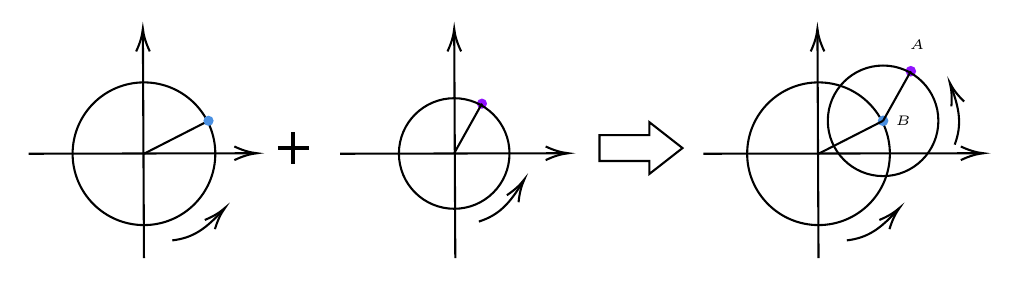
\begin{tikzpicture}[x=0.75pt,y=0.75pt,yscale=-1,xscale=1]
%uncomment if require: \path (0,300); %set diagram left start at 0, and has height of 300

%Straight Lines [id:da8777462388646522] 
\draw    (375,145.24) -- (508,145) ;
\draw [shift={(510,145)}, rotate = 179.9] [color={rgb, 255:red, 0; green, 0; blue, 0 }  ][line width=0.75]    (10.93,-3.29) .. controls (6.95,-1.4) and (3.31,-0.3) .. (0,0) .. controls (3.31,0.3) and (6.95,1.4) .. (10.93,3.29)   ;
%Straight Lines [id:da08971251069127839] 
\draw    (430.53,195.48) -- (430.01,87) ;
\draw [shift={(430,85)}, rotate = 89.73] [color={rgb, 255:red, 0; green, 0; blue, 0 }  ][line width=0.75]    (10.93,-3.29) .. controls (6.95,-1.4) and (3.31,-0.3) .. (0,0) .. controls (3.31,0.3) and (6.95,1.4) .. (10.93,3.29)   ;
%Shape: Ellipse [id:dp8343093110245612] 
\draw   (396.15,145.24) .. controls (396.15,126.25) and (411.54,110.86) .. (430.53,110.86) .. controls (449.51,110.86) and (464.9,126.25) .. (464.9,145.24) .. controls (464.9,164.22) and (449.51,179.61) .. (430.53,179.61) .. controls (411.54,179.61) and (396.15,164.22) .. (396.15,145.24) -- cycle ;
%Shape: Boxed Bezier Curve [id:dp20273047553204648] 
\draw    (444.17,186.98) .. controls (454.46,185.8) and (460.48,181.15) .. (468.36,172.64) ;
\draw [shift={(469.62,171.26)}, rotate = 132.21] [color={rgb, 255:red, 0; green, 0; blue, 0 }  ][line width=0.75]    (10.93,-3.29) .. controls (6.95,-1.4) and (3.31,-0.3) .. (0,0) .. controls (3.31,0.3) and (6.95,1.4) .. (10.93,3.29)   ;
%Shape: Ellipse [id:dp3900535515051158] 
\draw  [color={rgb, 255:red, 144; green, 19; blue, 254 }  ,draw opacity=1 ][fill={rgb, 255:red, 144; green, 19; blue, 254 }  ,fill opacity=1 ] (472.98,105.48) .. controls (472.98,104.36) and (473.88,103.45) .. (475,103.45) .. controls (476.12,103.45) and (477.02,104.36) .. (477.02,105.48) .. controls (477.02,106.59) and (476.12,107.5) .. (475,107.5) .. controls (473.88,107.5) and (472.98,106.59) .. (472.98,105.48) -- cycle ;
%Shape: Ellipse [id:dp6447307612664201] 
\draw  [color={rgb, 255:red, 74; green, 144; blue, 226 }  ,draw opacity=1 ][fill={rgb, 255:red, 74; green, 144; blue, 226 }  ,fill opacity=1 ] (459.61,129.37) .. controls (459.61,128.26) and (460.52,127.35) .. (461.63,127.35) .. controls (462.75,127.35) and (463.66,128.26) .. (463.66,129.37) .. controls (463.66,130.49) and (462.75,131.4) .. (461.63,131.4) .. controls (460.52,131.4) and (459.61,130.49) .. (459.61,129.37) -- cycle ;
%Straight Lines [id:da9814486294608644] 
\draw    (430.53,145.24) -- (461.63,129.37) ;
%Shape: Ellipse [id:dp8328575054736782] 
\draw   (435,129.37) .. controls (435,114.66) and (446.92,102.74) .. (461.63,102.74) .. controls (476.35,102.74) and (488.27,114.66) .. (488.27,129.37) .. controls (488.27,144.08) and (476.35,156.01) .. (461.63,156.01) .. controls (446.92,156.01) and (435,144.08) .. (435,129.37) -- cycle ;
%Straight Lines [id:da5174110342809759] 
\draw    (461.63,129.37) -- (474.04,107.2) -- (475,105.48) ;
%Shape: Boxed Bezier Curve [id:dp7196733208732373] 
\draw    (496.14,140.85) .. controls (499.79,131.15) and (498.4,123.68) .. (494.41,112.78) ;
\draw [shift={(493.76,111.03)}, rotate = 69.34] [color={rgb, 255:red, 0; green, 0; blue, 0 }  ][line width=0.75]    (10.93,-3.29) .. controls (6.95,-1.4) and (3.31,-0.3) .. (0,0) .. controls (3.31,0.3) and (6.95,1.4) .. (10.93,3.29)   ;
%Straight Lines [id:da21008655606312154] 
\draw    (50,145.24) -- (158,145) ;
\draw [shift={(160,145)}, rotate = 179.88] [color={rgb, 255:red, 0; green, 0; blue, 0 }  ][line width=0.75]    (10.93,-3.29) .. controls (6.95,-1.4) and (3.31,-0.3) .. (0,0) .. controls (3.31,0.3) and (6.95,1.4) .. (10.93,3.29)   ;
%Straight Lines [id:da3443268353047235] 
\draw    (105.53,195.48) -- (105.01,87) ;
\draw [shift={(105,85)}, rotate = 89.73] [color={rgb, 255:red, 0; green, 0; blue, 0 }  ][line width=0.75]    (10.93,-3.29) .. controls (6.95,-1.4) and (3.31,-0.3) .. (0,0) .. controls (3.31,0.3) and (6.95,1.4) .. (10.93,3.29)   ;
%Shape: Ellipse [id:dp8259321146716279] 
\draw   (71.15,145.24) .. controls (71.15,126.25) and (86.54,110.86) .. (105.53,110.86) .. controls (124.51,110.86) and (139.9,126.25) .. (139.9,145.24) .. controls (139.9,164.22) and (124.51,179.61) .. (105.53,179.61) .. controls (86.54,179.61) and (71.15,164.22) .. (71.15,145.24) -- cycle ;
%Shape: Boxed Bezier Curve [id:dp654429933459092] 
\draw    (119.17,186.98) .. controls (129.46,185.8) and (135.48,181.15) .. (143.36,172.64) ;
\draw [shift={(144.62,171.26)}, rotate = 132.21] [color={rgb, 255:red, 0; green, 0; blue, 0 }  ][line width=0.75]    (10.93,-3.29) .. controls (6.95,-1.4) and (3.31,-0.3) .. (0,0) .. controls (3.31,0.3) and (6.95,1.4) .. (10.93,3.29)   ;
%Straight Lines [id:da22397521775334828] 
\draw    (105.53,145.24) -- (136.63,129.37) ;
%Shape: Circle [id:dp22967192953498516] 
\draw  [color={rgb, 255:red, 144; green, 19; blue, 254 }  ,draw opacity=1 ][fill={rgb, 255:red, 144; green, 19; blue, 254 }  ,fill opacity=1 ] (266.45,121.1) .. controls (266.45,120.05) and (267.31,119.19) .. (268.37,119.19) .. controls (269.42,119.19) and (270.28,120.05) .. (270.28,121.1) .. controls (270.28,122.16) and (269.42,123.02) .. (268.37,123.02) .. controls (267.31,123.02) and (266.45,122.16) .. (266.45,121.1) -- cycle ;
%Shape: Circle [id:dp10062477997817343] 
\draw  [color={rgb, 255:red, 74; green, 144; blue, 226 }  ,draw opacity=1 ][fill={rgb, 255:red, 74; green, 144; blue, 226 }  ,fill opacity=1 ] (134.72,129.37) .. controls (134.72,128.32) and (135.58,127.46) .. (136.63,127.46) .. controls (137.69,127.46) and (138.55,128.32) .. (138.55,129.37) .. controls (138.55,130.43) and (137.69,131.29) .. (136.63,131.29) .. controls (135.58,131.29) and (134.72,130.43) .. (134.72,129.37) -- cycle ;
%Straight Lines [id:da18723751264672028] 
\draw    (200,145.24) -- (308,145) ;
\draw [shift={(310,145)}, rotate = 179.88] [color={rgb, 255:red, 0; green, 0; blue, 0 }  ][line width=0.75]    (10.93,-3.29) .. controls (6.95,-1.4) and (3.31,-0.3) .. (0,0) .. controls (3.31,0.3) and (6.95,1.4) .. (10.93,3.29)   ;
%Straight Lines [id:da3858540025010373] 
\draw    (255.53,195.48) -- (255.01,87) ;
\draw [shift={(255,85)}, rotate = 89.73] [color={rgb, 255:red, 0; green, 0; blue, 0 }  ][line width=0.75]    (10.93,-3.29) .. controls (6.95,-1.4) and (3.31,-0.3) .. (0,0) .. controls (3.31,0.3) and (6.95,1.4) .. (10.93,3.29)   ;
%Shape: Boxed Bezier Curve [id:dp38955918165168324] 
\draw    (266.9,177.91) .. controls (276.77,174.75) and (281.77,169.03) .. (287.85,159.14) ;
\draw [shift={(288.82,157.55)}, rotate = 121.02] [color={rgb, 255:red, 0; green, 0; blue, 0 }  ][line width=0.75]    (10.93,-3.29) .. controls (6.95,-1.4) and (3.31,-0.3) .. (0,0) .. controls (3.31,0.3) and (6.95,1.4) .. (10.93,3.29)   ;
%Shape: Ellipse [id:dp711443710802991] 
\draw   (228.36,145.12) .. controls (228.36,130.41) and (240.29,118.48) .. (255,118.48) .. controls (269.71,118.48) and (281.64,130.41) .. (281.64,145.12) .. controls (281.64,159.83) and (269.71,171.75) .. (255,171.75) .. controls (240.29,171.75) and (228.36,159.83) .. (228.36,145.12) -- cycle ;
%Straight Lines [id:da35780273242154625] 
\draw    (255,145) -- (267.4,122.82) -- (268.37,121.1) ;
\draw  [line width=1.5]  (170,142.5) -- (185,142.5)(177.5,135) -- (177.5,150) ;
%Right Arrow [id:dp968115258076975] 
\draw   (325,136.25) -- (349,136.25) -- (349,130) -- (365,142.5) -- (349,155) -- (349,148.75) -- (325,148.75) -- cycle ;

% Text Node
\draw (483,88.88) node [anchor=north east] [inner sep=0.75pt]  [font=\tiny]  {$A$};
% Text Node
\draw (466.12,129.37) node [anchor=west] [inner sep=0.75pt]  [font=\tiny]  {$B$};


\end{tikzpicture}

\end{center}

如图所示,现有两个参考圆,分别对应$x$轴的两个简谐振动,若这两个简谐运动叠加可得到一个新的运动,此运动可以等效为这两个参考圆首尾相连后末端$A$点在$x$轴方向的投影的运动。此方法在考试中很少碰到,在此不做过多介绍。

\section{“同侧法”判断波动方向}

\begin{center}

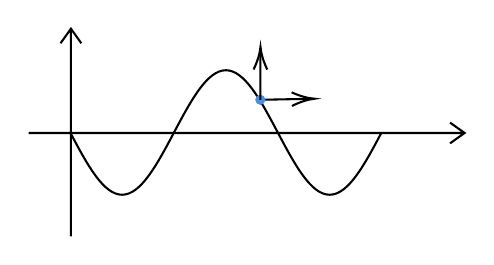
\begin{tikzpicture}[x=0.75pt,y=0.75pt,yscale=-1,xscale=1]
%uncomment if require: \path (0,300); %set diagram left start at 0, and has height of 300

%Shape: Axis 2D [id:dp17044305030121132] 
\draw  (70,150.23) -- (280,150.23)(90.34,100) -- (90.34,200) (273,145.23) -- (280,150.23) -- (273,155.23) (85.34,107) -- (90.34,100) -- (95.34,107)  ;
%Shape: Wave [id:dp3213186683813747] 
\draw   (90,150) .. controls (98.15,165.37) and (105.95,180) .. (115,180) .. controls (124.05,180) and (131.85,165.37) .. (140,150) .. controls (148.15,134.63) and (155.95,120) .. (165,120) .. controls (174.05,120) and (181.85,134.63) .. (190,150) .. controls (198.15,165.37) and (205.95,180) .. (215,180) .. controls (224.05,180) and (231.85,165.37) .. (240,150) ;
%Straight Lines [id:da4960855789495031] 
\draw    (181.58,134.25) -- (205.67,133.77) ;
\draw [shift={(207.67,133.73)}, rotate = 178.86] [color={rgb, 255:red, 0; green, 0; blue, 0 }  ][line width=0.75]    (10.93,-3.29) .. controls (6.95,-1.4) and (3.31,-0.3) .. (0,0) .. controls (3.31,0.3) and (6.95,1.4) .. (10.93,3.29)   ;
%Shape: Circle [id:dp4675822922340589] 
\draw  [color={rgb, 255:red, 74; green, 144; blue, 226 }  ,draw opacity=1 ][fill={rgb, 255:red, 74; green, 144; blue, 226 }  ,fill opacity=1 ] (179.67,134.25) .. controls (179.67,133.19) and (180.52,132.33) .. (181.58,132.33) .. controls (182.64,132.33) and (183.49,133.19) .. (183.49,134.25) .. controls (183.49,135.3) and (182.64,136.16) .. (181.58,136.16) .. controls (180.52,136.16) and (179.67,135.3) .. (179.67,134.25) -- cycle ;
%Straight Lines [id:da7406502193343325] 
\draw    (181.58,134.25) -- (181.66,110.73) ;
\draw [shift={(181.67,108.73)}, rotate = 90.2] [color={rgb, 255:red, 0; green, 0; blue, 0 }  ][line width=0.75]    (10.93,-3.29) .. controls (6.95,-1.4) and (3.31,-0.3) .. (0,0) .. controls (3.31,0.3) and (6.95,1.4) .. (10.93,3.29)   ;

\end{tikzpicture}

\end{center}

一简谐波的波形图($y - x$图)如上图所示,上有一质点,判断波的传播方向或该质点此时的运动方向有如下简便的方法。

\begin{theo}{“同侧法”判断波动方向}{}
任取一个\textbf{非顶点}的质点,左右传播方向和该质点运动方向成一个九十度角。如图所示可以用两个剪头分别表示出来。\textbf{在波形图中,这两个箭头一定是在波的同侧出现。}

运用此方法,知道波的振动方向或某时刻质点的运动方向,便可快速判读出另一个方向。

\end{theo}

\section{“旋转法”判断干涉平面凸起还是凹下}

\begin{center}


\tikzset{every picture/.style={line width=0.75pt}} %set default line width to 0.75pt        

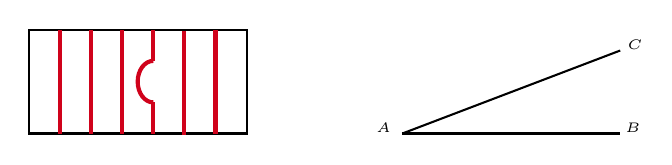
\begin{tikzpicture}[x=0.75pt,y=0.75pt,yscale=-1,xscale=1]
%uncomment if require: \path (0,300); %set diagram left start at 0, and has height of 300

%Shape: Rectangle [id:dp5450967430811406] 
\draw   (65,75) -- (170,75) -- (170,125) -- (65,125) -- cycle ;
%Straight Lines [id:da7207554445840463] 
\draw [color={rgb, 255:red, 208; green, 2; blue, 27 }  ,draw opacity=1 ][line width=1.5]    (80,75) -- (80,125) ;
%Straight Lines [id:da8856015597811548] 
\draw [color={rgb, 255:red, 208; green, 2; blue, 27 }  ,draw opacity=1 ][line width=1.5]    (95,75) -- (95,125) ;
%Straight Lines [id:da27302137833179474] 
\draw [color={rgb, 255:red, 208; green, 2; blue, 27 }  ,draw opacity=1 ][line width=1.5]    (110,75) -- (110,125) ;
%Straight Lines [id:da2045981797610763] 
\draw [color={rgb, 255:red, 208; green, 2; blue, 27 }  ,draw opacity=1 ][line width=1.5]    (125,110) -- (125,125) ;
%Straight Lines [id:da1792503962330343] 
\draw [color={rgb, 255:red, 208; green, 2; blue, 27 }  ,draw opacity=1 ][line width=1.5]    (140,75.5) -- (140,125.5) ;
%Straight Lines [id:da9645464264966506] 
\draw [color={rgb, 255:red, 208; green, 2; blue, 27 }  ,draw opacity=1 ][line width=1.5]    (155,75) -- (155,125) ;
%Straight Lines [id:da853883505351509] 
\draw [color={rgb, 255:red, 208; green, 2; blue, 27 }  ,draw opacity=1 ][line width=1.5]    (125,75) -- (125,90) ;
%Shape: Arc [id:dp6231057404985074] 
\draw  [draw opacity=0][line width=1.5]  (125,110) .. controls (120.86,110) and (117.5,105.52) .. (117.5,100) .. controls (117.5,94.48) and (120.86,90) .. (125,90) -- (125,100) -- cycle ; \draw  [color={rgb, 255:red, 208; green, 2; blue, 27 }  ,draw opacity=1 ][line width=1.5]  (125,110) .. controls (120.86,110) and (117.5,105.52) .. (117.5,100) .. controls (117.5,94.48) and (120.86,90) .. (125,90) ;  
%Straight Lines [id:da4819698726867141] 
\draw    (245,125) -- (350,125) ;
%Straight Lines [id:da2187262824312195] 
\draw    (245,125) -- (350,85) ;

% Text Node
\draw (231,118.4) node [anchor=north west][inner sep=0.75pt]  [font=\tiny]  {$A$};
% Text Node
\draw (351,118.4) node [anchor=north west][inner sep=0.75pt]  [font=\tiny]  {$B$};
% Text Node
\draw (352,78.4) node [anchor=north west][inner sep=0.75pt]  [font=\tiny]  {$C$};


\end{tikzpicture}

\end{center}

如右图所示,现用一块平整的玻璃板$AC$与待测板$AB$形成一劈尖,并用激光照射,其干涉图样如左图所示,现判断待测板存在凸起还是凹陷。

对于这类题目,我们可以想象\textbf{将干涉条纹“叠加”到劈尖上,并“旋转”劈尖使得尖端指向自己},如图所示。

\begin{center}


\tikzset{every picture/.style={line width=0.75pt}} %set default line width to 0.75pt        

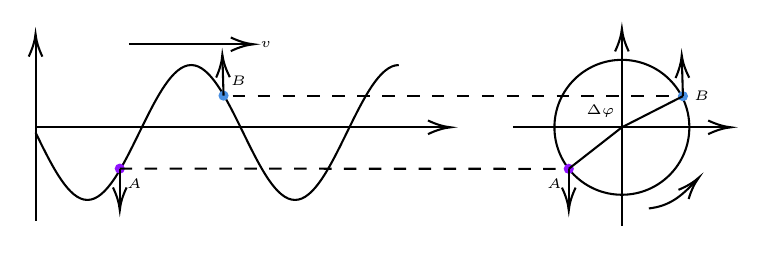
\begin{tikzpicture}[x=0.75pt,y=0.75pt,yscale=-1,xscale=1]
%uncomment if require: \path (0,300); %set diagram left start at 0, and has height of 300

%Straight Lines [id:da7017512425586769] 
\draw    (105,85) -- (303,85) ;
\draw [shift={(305,85)}, rotate = 180] [color={rgb, 255:red, 0; green, 0; blue, 0 }  ][line width=0.75]    (10.93,-3.29) .. controls (6.95,-1.4) and (3.31,-0.3) .. (0,0) .. controls (3.31,0.3) and (6.95,1.4) .. (10.93,3.29)   ;
%Straight Lines [id:da6617890815314416] 
\draw    (105,130) -- (105,42) ;
\draw [shift={(105,40)}, rotate = 90] [color={rgb, 255:red, 0; green, 0; blue, 0 }  ][line width=0.75]    (10.93,-3.29) .. controls (6.95,-1.4) and (3.31,-0.3) .. (0,0) .. controls (3.31,0.3) and (6.95,1.4) .. (10.93,3.29)   ;
%Shape: Wave [id:dp8842981491970783] 
\draw   (105,87.5) .. controls (113.15,104.15) and (120.95,120) .. (130,120) .. controls (139.05,120) and (146.85,104.15) .. (155,87.5) .. controls (163.15,70.85) and (170.95,55) .. (180,55) .. controls (189.05,55) and (196.85,70.85) .. (205,87.5) .. controls (213.15,104.15) and (220.95,120) .. (230,120) .. controls (239.05,120) and (246.85,104.15) .. (255,87.5) .. controls (263.15,70.85) and (270.95,55) .. (280,55) ;
%Straight Lines [id:da8040591192782738] 
\draw    (150,45) -- (208,45) ;
\draw [shift={(210,45)}, rotate = 180] [color={rgb, 255:red, 0; green, 0; blue, 0 }  ][line width=0.75]    (10.93,-3.29) .. controls (6.95,-1.4) and (3.31,-0.3) .. (0,0) .. controls (3.31,0.3) and (6.95,1.4) .. (10.93,3.29)   ;
%Shape: Circle [id:dp5419707917308172] 
\draw  [color={rgb, 255:red, 74; green, 144; blue, 226 }  ,draw opacity=1 ][fill={rgb, 255:red, 74; green, 144; blue, 226 }  ,fill opacity=1 ] (193.67,69.75) .. controls (193.67,68.69) and (194.52,67.83) .. (195.58,67.83) .. controls (196.64,67.83) and (197.49,68.69) .. (197.49,69.75) .. controls (197.49,70.8) and (196.64,71.66) .. (195.58,71.66) .. controls (194.52,71.66) and (193.67,70.8) .. (193.67,69.75) -- cycle ;
%Shape: Circle [id:dp681644701248078] 
\draw  [color={rgb, 255:red, 144; green, 19; blue, 254 }  ,draw opacity=1 ][fill={rgb, 255:red, 144; green, 19; blue, 254 }  ,fill opacity=1 ] (143.67,104.91) .. controls (143.67,103.86) and (144.53,103) .. (145.59,103) .. controls (146.64,103) and (147.5,103.86) .. (147.5,104.91) .. controls (147.5,105.97) and (146.64,106.83) .. (145.59,106.83) .. controls (144.53,106.83) and (143.67,105.97) .. (143.67,104.91) -- cycle ;
%Straight Lines [id:da8371978854765523] 
\draw    (335,85) -- (438,85) ;
\draw [shift={(440,85)}, rotate = 180] [color={rgb, 255:red, 0; green, 0; blue, 0 }  ][line width=0.75]    (10.93,-3.29) .. controls (6.95,-1.4) and (3.31,-0.3) .. (0,0) .. controls (3.31,0.3) and (6.95,1.4) .. (10.93,3.29)   ;
%Straight Lines [id:da01679847276348334] 
\draw    (387.5,132.5) -- (387.5,39.5) ;
\draw [shift={(387.5,37.5)}, rotate = 90] [color={rgb, 255:red, 0; green, 0; blue, 0 }  ][line width=0.75]    (10.93,-3.29) .. controls (6.95,-1.4) and (3.31,-0.3) .. (0,0) .. controls (3.31,0.3) and (6.95,1.4) .. (10.93,3.29)   ;
%Shape: Circle [id:dp05496182766044977] 
\draw   (355,85) .. controls (355,67.05) and (369.55,52.5) .. (387.5,52.5) .. controls (405.45,52.5) and (420,67.05) .. (420,85) .. controls (420,102.95) and (405.45,117.5) .. (387.5,117.5) .. controls (369.55,117.5) and (355,102.95) .. (355,85) -- cycle ;
%Shape: Boxed Bezier Curve [id:dp4427700767601117] 
\draw    (400.49,124.09) .. controls (410.17,122.98) and (415.85,118.63) .. (423.25,110.66) ;
\draw [shift={(424.56,109.23)}, rotate = 132.21] [color={rgb, 255:red, 0; green, 0; blue, 0 }  ][line width=0.75]    (10.93,-3.29) .. controls (6.95,-1.4) and (3.31,-0.3) .. (0,0) .. controls (3.31,0.3) and (6.95,1.4) .. (10.93,3.29)   ;
%Straight Lines [id:da12057449898734451] 
\draw  [dash pattern={on 4.5pt off 4.5pt}]  (145.59,104.91) -- (360,105) ;
%Straight Lines [id:da8953406033575979] 
\draw  [dash pattern={on 4.5pt off 4.5pt}]  (200,70) -- (416.91,70) ;
%Shape: Circle [id:dp0790887111106604] 
\draw  [color={rgb, 255:red, 144; green, 19; blue, 254 }  ,draw opacity=1 ][fill={rgb, 255:red, 144; green, 19; blue, 254 }  ,fill opacity=1 ] (360,105) .. controls (360,103.94) and (360.86,103.09) .. (361.91,103.09) .. controls (362.97,103.09) and (363.83,103.94) .. (363.83,105) .. controls (363.83,106.06) and (362.97,106.91) .. (361.91,106.91) .. controls (360.86,106.91) and (360,106.06) .. (360,105) -- cycle ;
%Shape: Circle [id:dp9734580095926755] 
\draw  [color={rgb, 255:red, 74; green, 144; blue, 226 }  ,draw opacity=1 ][fill={rgb, 255:red, 74; green, 144; blue, 226 }  ,fill opacity=1 ] (415,70) .. controls (415,68.94) and (415.86,68.09) .. (416.91,68.09) .. controls (417.97,68.09) and (418.83,68.94) .. (418.83,70) .. controls (418.83,71.06) and (417.97,71.91) .. (416.91,71.91) .. controls (415.86,71.91) and (415,71.06) .. (415,70) -- cycle ;
%Straight Lines [id:da5425744113579352] 
\draw    (145.59,104.91) -- (145.59,122.91) ;
\draw [shift={(145.59,124.91)}, rotate = 270] [color={rgb, 255:red, 0; green, 0; blue, 0 }  ][line width=0.75]    (10.93,-3.29) .. controls (6.95,-1.4) and (3.31,-0.3) .. (0,0) .. controls (3.31,0.3) and (6.95,1.4) .. (10.93,3.29)   ;
%Straight Lines [id:da30567757197948686] 
\draw    (195.58,69.75) -- (195.06,52) ;
\draw [shift={(195,50)}, rotate = 88.32] [color={rgb, 255:red, 0; green, 0; blue, 0 }  ][line width=0.75]    (10.93,-3.29) .. controls (6.95,-1.4) and (3.31,-0.3) .. (0,0) .. controls (3.31,0.3) and (6.95,1.4) .. (10.93,3.29)   ;
%Straight Lines [id:da038712253350430936] 
\draw    (361.91,105) -- (361.91,123) ;
\draw [shift={(361.91,125)}, rotate = 270] [color={rgb, 255:red, 0; green, 0; blue, 0 }  ][line width=0.75]    (10.93,-3.29) .. controls (6.95,-1.4) and (3.31,-0.3) .. (0,0) .. controls (3.31,0.3) and (6.95,1.4) .. (10.93,3.29)   ;
%Shape: Boxed Line [id:dp41235110909485106] 
\draw    (416.91,70) -- (416.39,52.25) ;
\draw [shift={(416.33,50.25)}, rotate = 88.32] [color={rgb, 255:red, 0; green, 0; blue, 0 }  ][line width=0.75]    (10.93,-3.29) .. controls (6.95,-1.4) and (3.31,-0.3) .. (0,0) .. controls (3.31,0.3) and (6.95,1.4) .. (10.93,3.29)   ;
%Straight Lines [id:da38275778119556225] 
\draw    (361.91,105) -- (387.5,85) ;
%Straight Lines [id:da6622505808590617] 
\draw    (387.5,85) -- (416.91,70) ;

% Text Node
\draw (212,45) node [anchor=west] [inner sep=0.75pt]  [font=\tiny]  {$v$};
% Text Node
\draw (385.5,81.6) node [anchor=south east] [inner sep=0.75pt]  [font=\tiny]  {$\Delta \varphi $};
% Text Node
\draw (147.59,108.31) node [anchor=north west][inner sep=0.75pt]  [font=\tiny]  {$A$};
% Text Node
\draw (359.91,108.4) node [anchor=north east] [inner sep=0.75pt]  [font=\tiny]  {$A$};
% Text Node
\draw (197.58,66.35) node [anchor=south west] [inner sep=0.75pt]  [font=\tiny]  {$B$};
% Text Node
\draw (420.83,70) node [anchor=west] [inner sep=0.75pt]  [font=\tiny]  {$B$};


\end{tikzpicture}

\end{center}

在进行这样的想象后,若干涉条纹向下凹,则待测板凹陷,反之若干涉条纹向上凸,则待测板凸起。此过程非常直观,劈尖摆放向左或向右均可使用,可快速判断此类问题。

\begin{mk}{易错提醒}{}
一般而言,题目中\textbf{倾斜放置的是标准板,而水平放置的是待测板},且\textbf{一般从上方向下观察条纹}。目前笔者并未见到其他情形的题目,但\textbf{若出现除上述情形之外的情形,则需要具体问题具体讨论}。笔者并未验证过其他情况的正确性。
~\\

条纹的弯曲\textbf{本质上是光程差的偏大或偏小},或许可以总结出条纹弯曲与光程差偏大或偏小的更通用的结论,读者可以自行总结和探讨。
\end{mk}

\section{双缝干涉 —— “横乘横等于竖乘竖”}

\begin{center}



\tikzset{every picture/.style={line width=0.75pt}} %set default line width to 0.75pt        

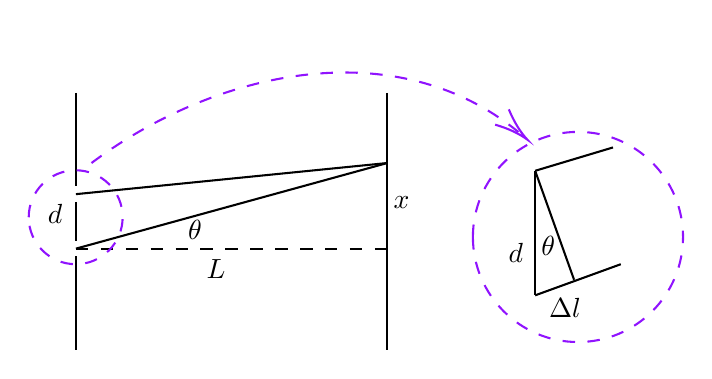
\begin{tikzpicture}[x=0.75pt,y=0.75pt,yscale=-1.5,xscale=1.5]
%uncomment if require: \path (0,300); %set diagram left start at 0, and has height of 300

%Straight Lines [id:da7937139484326525] 
\draw    (130,55) -- (130,85) ;
%Straight Lines [id:da5514747070310864] 
\draw    (130,90) -- (130,102.5) ;
%Straight Lines [id:da3180465848105889] 
\draw    (130,107.5) -- (130,137.5) ;
%Straight Lines [id:da26896276424224896] 
\draw    (230,55) -- (230,137.5) ;
%Straight Lines [id:da7167210011053942] 
\draw  [dash pattern={on 4.5pt off 4.5pt}]  (130,105) -- (230,105) ;
%Straight Lines [id:da7138419970578529] 
\draw    (130,105) -- (230,77.5) ;
%Straight Lines [id:da7800441168755299] 
\draw    (130,87.5) -- (230,77.5) ;
%Shape: Circle [id:dp49969692270722277] 
\draw  [color={rgb, 255:red, 144; green, 19; blue, 254 }  ,draw opacity=1 ][dash pattern={on 4.5pt off 4.5pt}] (114.83,94.92) .. controls (114.83,86.58) and (121.58,79.83) .. (129.92,79.83) .. controls (138.25,79.83) and (145,86.58) .. (145,94.92) .. controls (145,103.25) and (138.25,110) .. (129.92,110) .. controls (121.58,110) and (114.83,103.25) .. (114.83,94.92) -- cycle ;
%Curve Lines [id:da6541923848279152] 
\draw [color={rgb, 255:red, 144; green, 19; blue, 254 }  ,draw opacity=1 ] [dash pattern={on 4.5pt off 4.5pt}]  (135,77.5) .. controls (174.6,47.8) and (233.56,34.36) .. (273.79,68.94) ;
\draw [shift={(275,70)}, rotate = 221.74] [color={rgb, 255:red, 144; green, 19; blue, 254 }  ,draw opacity=1 ][line width=0.75]    (10.93,-3.29) .. controls (6.95,-1.4) and (3.31,-0.3) .. (0,0) .. controls (3.31,0.3) and (6.95,1.4) .. (10.93,3.29)   ;
%Straight Lines [id:da18744774929107222] 
\draw    (277.5,80) -- (302.5,72.5) ;
%Straight Lines [id:da2397390109705031] 
\draw    (277.5,120) -- (305,110) ;
%Straight Lines [id:da21304007677005732] 
\draw    (277.5,80) -- (277.5,120) ;
%Straight Lines [id:da6975177627780123] 
\draw    (277.5,80) -- (290,115) ;
%Shape: Circle [id:dp9982306358023718] 
\draw  [color={rgb, 255:red, 144; green, 19; blue, 254 }  ,draw opacity=1 ][dash pattern={on 4.5pt off 4.5pt}] (257.5,101.25) .. controls (257.5,82.61) and (272.61,67.5) .. (291.25,67.5) .. controls (309.89,67.5) and (325,82.61) .. (325,101.25) .. controls (325,119.89) and (309.89,135) .. (291.25,135) .. controls (272.61,135) and (257.5,119.89) .. (257.5,101.25) -- cycle ;

% Text Node
\draw (171,107.4) node [anchor=north west][inner sep=0.75pt]  [font=\normalsize]  {$L$};
% Text Node
\draw (120,89.9) node [anchor=north west][inner sep=0.75pt]  [font=\normalsize]  {$d$};
% Text Node
\draw (231,87.4) node [anchor=north west][inner sep=0.75pt]  [font=\normalsize]  {$x$};
% Text Node
\draw (268,102.4) node [anchor=north west][inner sep=0.75pt]  [font=\normalsize]  {$d$};
% Text Node
\draw (165,95) node [anchor=north west][inner sep=0.75pt]  [font=\normalsize]  {$\theta $};
% Text Node
\draw (278.5,100) node [anchor=north west][inner sep=0.75pt]  [font=\normalsize]  {$\theta $};
% Text Node
\draw (281,119.9) node [anchor=north west][inner sep=0.75pt]  [font=\normalsize]  {$\Delta l$};


\end{tikzpicture}

\end{center}

如图,一个间距为$d$的双缝,离光屏距离为$L$,干涉条纹间距为$\Delta x$,光的波长为$\lambda$。\textbf{由于光屏比较远(即满足$L \gg d$),则可以近似认为从双缝发出的光到光屏上同一点的光线互相平行}。

记到某一点的两束光光程差为$\Delta l$,第$n$条亮条纹离光屏上的等光程点距离为$x_n$(根据前文近似条件,这里取下面的缝发出光线垂直于光屏时的位置为等光程点\footnote{当然这里也可以取上面的缝对应在光屏上的点或者两缝中点对应在光屏上的点,由于$d$为小量,可以略去不同取法的差别}。)由几何关系,有

$$ \Delta l = d \sin \theta $$
$$ x_n = L \tan \theta $$

由于亮条纹光程差满足$\Delta l = n \lambda$($n \in \mathbb{N^{+}}$),故

\begin{subequations}
\begin{align*}
x_n = L \tan \theta \tikzmarknode{xljs}{\highlight{red}{$\approx L \sin \theta$}} = \frac{L \Delta l}{d} = \frac{n \lambda L}{d}
\end{align*}
\end{subequations}

\begin{tikzpicture}[overlay,remember picture,>=stealth,nodes={align=left,inner ysep=1pt},<-]

\path (xljs.south) ++ (0,-2em) node[anchor=north] (xljsscalep){\highlight{red}{$\theta$为小量时,$\theta \approx \sin \theta \approx \tan \theta$(见“常用小量近似”\eqref{s_xljs})}};
\draw [color=red!87](xljs.south) -- ([color=red]xljsscalep.north);

\end{tikzpicture}

\vspace{2\baselineskip}
因此,两条亮条纹之间间距$\Delta x = x_n - x_{n-1} = \frac{\lambda L}{d}$,故

\begin{theo}{双缝干涉 —— “横乘横等于竖乘竖”}{}
在双缝干涉中,干涉条纹间距$\Delta x$、双缝距离$d$、缝与光屏距离$L$、光的波长$\lambda$满足

$$L \lambda = d \Delta x$$

记忆方法为\textbf{“横乘横等于竖乘竖”}(光为横波,故光的波长记为“横”,乘上“横的距离”(即为$L$,在示意图中它是“横着的”),等于两个“竖的距离”相乘(即为$d$和$\Delta x$,在示意图中它是“竖着的”))
\end{theo}


%\subsection{}
